% main.tex: generated campaign report, quantum-history, run 20260910T085020Z.
%
% Written by hte.paper.emit_paper from this run's own artifacts
% (MANIFEST.json, timeline.json, calibration.json, self-report.json under
% runs/quantum-history/20260910T085020Z). Load order, biblatex then hyperref then bucket.sty, and every
% other convention here follow papers/PAPER-STANDARDS.md; papers/template/
% is this file's own starting point.
\documentclass[11pt]{article}

\usepackage[margin=1in]{geometry}
\usepackage[T1]{fontenc}
\usepackage{csquotes}

\usepackage[backend=biber,style=numeric,sorting=none,maxnames=3,minnames=1]{biblatex}
\addbibresource{refs.bib}
\addbibresource{/home/gian/agfarms/bucket-foundation/papers/bib/common.bib}

\usepackage{hyperref}

\usepackage{bucket}

\hypersetup{
  colorlinks = true,
  linkcolor  = bucketblue,
  citecolor  = bucketblue,
  urlcolor   = bucketblue,
}

\glossentry{opinion}{opinion}%
  {https://github.com/AGFarms/bucket-foundation/blob/master/tools/hypothesis-engine/hte/belief.py}%
  {A subjective-logic opinion $(b, d, u, a)$: belief, disbelief, uncertainty mass, and base rate, fused from pooled supporting and refuting evidence weight against a total-ignorance constant $W$.}

\glossentry{posterior}{projected posterior}%
  {https://github.com/AGFarms/bucket-foundation/blob/master/tools/hypothesis-engine/hte/belief.py}%
  {$P(h) = b(h) + a(h) \cdot u(h)$, an opinion's single-number projection, used to rank hypotheses within a time bin.}

\glossentry{missingmass}{missing mass}%
  {https://github.com/AGFarms/bucket-foundation/blob/master/tools/hypothesis-engine/hte/unknowns.py}%
  {The Good-Turing estimate of the address-space share made of hypotheses observed exactly once across a campaign's generation seeds.}

\glossentry{targetblind}{target-blind}%
  {https://github.com/AGFarms/bucket-foundation/blob/master/tools/hypothesis-engine/hte/runner.py}%
  {A generation or judging pass that applies the identical standard regardless of whether the reading under test is the consensus or a fringe one; tracked run over run as the non-consensus actor/mechanism proposal rate.}

\glossentry{coverageinterval}{coverage interval}%
  {https://github.com/AGFarms/bucket-foundation/blob/master/tools/hypothesis-engine/hte/unknowns.py}%
  {A Chao1-based 95\% band on how much of the address space this campaign's generation seeds have observed, \texttt{hte.unknowns.coverage\_interval}.}

\title{Quantum History: An Automated Hypothesis-Engine Campaign}
\author{Bucket Foundation}
\date{2026-09-10}

\begin{document}
\maketitle

\begin{abstract}
We report one automated run of the Bucket Foundation history hypothesis engine \autocite{bkthte2026design} over the Quantum History corpus, with no human editing any hypothesis, evidence item, or score. From 16 sources and 161 evidence items, the engine generated 5990 distinct hypothesis addresses and carried 176 past its critic filter to scoring and the ranking tournament. A Chao1 coverage estimate over the generation seeds put the observed share of the address space at 0.023 to 0.031, with a Good-Turing missing-mass estimate of 0.040. 100.000\% of survivors held a stable projected probability across the four prior-belief profiles this package ships. A k-fold holdout over 105 held-out ground-truth events (17 covered by this run's own pre-holdout evidence) scored a Brier score of 0.423. The generator's own target-blind check reported a non-consensus actor or mechanism proposal rate of 0.950 (steady against the previous run). We state every number in this report from the run's own persisted artifacts, and list where those artifacts stop short of a full per-hypothesis accounting in \Cref{sec:limitations}.
\end{abstract}

\section{Introduction}
\label{sec:intro}

One run of the Bucket Foundation history hypothesis engine produced
every result below, campaign \texttt{quantum-history}, run id
\texttt{20260910T085020Z}, with no step in the run editing a hypothesis,
evidence item, or score by hand. \Cref{sec:method} names the
engine-loop stages this run executed and their config; \Cref{sec:results}
and \Cref{sec:calibration} state every quantitative outcome;
\Cref{sec:limitations} names what this run's own artifacts do not
carry.

\section{Related work}
\label{sec:related}

The design and every definition this report depends on, the address
space, the subjective-logic belief model, structural unknowns, and the
engine loop itself, are stated and proved once, in the companion
design paper \autocite{bkthte2026design}; this report adds no new
definition of its own. The belief model's own subjective-logic
foundation is Josang's \autocite{josang2016subjective}.

\section{Preliminaries}
\label{sec:prelim}

Every term below is defined in full in the design paper's own
Preliminaries and proved in its Lean listings; this section links each
one to the module that implements it rather than restating the
definition. An \term{opinion}{opinion} $(b, d, u, a)$ projects to a
single \term{posterior}{posterior} $P(h) = b + a u$. A campaign's
\term{missingmass}{missing mass} and \term{coverageinterval}{coverage
interval} come from a Chao1 estimate over its generation seeds. A
\term{targetblind}{target-blind} check compares this run's own
non-consensus proposal rate against the run before it.

\section{Method}
\label{sec:method}

This report's own campaign follows the engine loop the design paper diagrams \autocite{bkthte2026design}: corpus ingestion, an optional extraction-ensemble pass, vocabulary growth from the unknown-unknown role, a combinatorial-plus-evidence-driven generation pass repeated across a fixed number of seeds, an LLM critic filter, a preservation critique against the shipped detectability table, subjective-logic belief scoring \autocite{josang2016subjective}, a Swiss-style ranking tournament, robustness and surprise measurement across four prior-belief profiles, a Chao1 coverage estimate over the generation seeds, an optional discovery-date holdout calibration, and a self-report closing the run.

An extraction ensemble of three independent passes ran once over this corpus's first document (\texttt{\_CHAPTER}), producing 5 evidence items at an agreement score of 0.200 after escalating to the ensemble adjudicator.

This run used 3 generation seeds, 20 LLM-proposed placements per seed, a combinatorial sweep capped at 150 items per seed, a 400-hypothesis cap into scoring, 2 tournament rounds, and not recorded-level time resolution. \Cref{tab:models} lists which model backed each engine-loop role for this run.

\begin{table}[htbp]
  \centering
  \caption{Model backing each engine-loop role for this run.}
  \label{tab:models}
  \begin{tabular}{@{}ll@{}}
    \toprule
    Role & Model \\
    \midrule
    critic & \texttt{sonnet} \\
    extractor & \texttt{haiku} \\
    generator & \texttt{sonnet} \\
    judge & \texttt{sonnet} \\
    meta\_review & \texttt{sonnet} \\
    preservation\_critic & \texttt{sonnet} \\
    referee & \texttt{sonnet} \\
    self\_report & \texttt{sonnet} \\
    unknown\_unknown & \texttt{sonnet} \\
    \bottomrule
  \end{tabular}
\end{table}

\section{Results}
\label{sec:results}

\Cref{tab:bins} lists, for every time bin this run scored, how many placement hypotheses ranked into it and the highest-posterior survivor found there. \Cref{fig:bin-topk} plots the full top-$k$ posterior ranking per bin, and \Cref{fig:opinion-hist} plots the projected-posterior distribution across every distinct survivor these bins name. Beyond the per-bin view, this run's survivors resolved into 40 competing-placement event groups (hypotheses sharing an object and place) and 0 competing-sequence pair groups.

The unknown-unknown role grew the vocabulary by 12 concepts this run (3 action, 4 actor, 2 mechanism, 2 object, 1 place). The Chao1 coverage estimate over this run's generation seeds put the observed hypothesis count at 5990 against a Chao1 estimate of 226770.0, a missing-mass estimate of 0.040, and a 95\% coverage band of [0.023, 0.031].

\Cref{tab:robustness} summarizes robustness across the four prior-belief profiles (\texttt{consensus}, \texttt{skeptic}, \texttt{fringe}, \texttt{uniform}); the underlying per-hypothesis projections are not themselves persisted by this run (\Cref{sec:limitations}), so only the aggregate stable/unstable split is reported. The surprise rate, evidence naming no address any survivor materialized, was 0.130 (21 of 161 evidence items, by the same reasoning).

The evolver's meta-review pass, reading this run's whole survivor population and its opinions at once, reported the following. This is the role's own output, quoted verbatim: paraphrasing a model's structural read of its own run risks losing the detail a meta-review pass exists to surface.
% voice-ignore-next 40
\begin{quote}\small
\begin{verbatim}
The 176-hypothesis frontier looks diverse at the slot level (13+ actions, several mechanisms, ~15 places, a wide interval spread from 1900-2009) but this diversity is largely cosmetic. Opinion vectors repeat to many decimal places across dozens of hypotheses that differ only in 'action' or 'object' (e.g. all 13 Planck/1900/blackbody-spectrum/quantization variants share b=0.0664, d=0.9238 regardless of whether Planck 'quantized', 'proved', 'proposed', 'published', or 'uu-awarded-a-prize'), indicating the evaluator's output is effectively a lookup keyed on (actor, place, mechanism, interval) rather than genuinely sensitive to what action/object is claimed. Two structural artifacts stand out only in aggregate: (1) the 'a' (authority/base-rate) parameter takes a small fixed set of sigmoid-like constants that track actor identity almost 1:1 (mainstream physicists ~0.88-0.92, corporate/mystic 'fringe' actors like vendor-marketing and quantum-mysticism-popularizers ~0.002-0.27), so no hypothesis ever lets specific evidence override the actor-identity prior; (2) belief (b) never exceeds ~0.15 anywhere in the frontier except one mega-cluster keyed on place='solvay-brussels' + interval=[1927,2009] (an 82-year span), where b jumps to ~0.44-0.54 uniformly regardless of object plausibility - even for anachronistic pairings (Einstein/Heisenberg-Schrodinger + shors-algorithm, no-cloning-theorem, willow-below-threshold-result at 'Solvay 1927-2009'). This looks like an interval-width/place artifact rather than content-driven belief, and it is being recombined indiscriminately across implausible objects instead of being stress-tested. Uncertainty (u) is essentially flat at ~0.009-0.012 across the entire population regardless of period, source density, or anachronism risk - the engine never produces a genuine high-uncertainty ('we don't know') reading. Exploration depth is also asymmetric: Einstein gets exhaustive action-verb permutation for EPR/Solvay narratives (30+ variants, almost all at princeton-ias, all landing in the same low-to-moderate belief band), while alternative actors for the same events (Bohr, Heisenberg-Schrodinger, Podolsky/Rosen-equivalent) get only 1-4 shallow 'other-action' instances, and alternative places for Planck-1900/EPR-1935 are mostly left as generic 'other-place'/'unknown-place' or single-instance afterthoughts rather than historically specific or deeply explored. Net effect: the population presents surface-level slot variation but has converged on a narrow set of opinion clusters, with no branch expressing strong confident belief backed by content-specific reasoning, no branch expressing high genuine uncertainty, and no branch where a low-authority actor or an unconventional place/mechanism combination is allowed to earn high belief from evidence.

Flags:
- Opinion collapse / lookup-table degeneracy: dozens of hypotheses that differ only in 'action' or 'object' produce numerically identical (to many decimals) b/d/u triples, meaning those slots are cosmetically varied but not actually discriminating in the evaluation - the action/object dimensions are not being genuinely tested.
- Actor-locked authority prior: the 'a' parameter is drawn from a small fixed set of values that map almost 1:1 to actor identity (mainstream physicists always ~0.88-0.92, corporate/fringe actors always ~0.002-0.27); no hypothesis decouples authority from actor identity, so the population never explores 'fringe actor turns out credible' or 'mainstream actor's specific claim is weak'.
- Belief ceiling with one gamed exception: virtually the entire frontier is disbelief-dominated (b<0.15) except a place='solvay-brussels'+interval=[1927,2009] mega-cluster where b~0.44-0.54; this 82-year interval boost applies almost uniformly across wildly different (including anachronistic) objects, suggesting an interval-width/place artifact rather than genuine evidential support, and it is unexamined - no sub-interval splits test whether the belief survives narrowing the window.
- Flat uncertainty: u sits at ~0.009-0.012 for essentially all 176 hypotheses regardless of period, source density, or plausibility - the population never generates a high-uncertainty 'genuinely unresolved' reading, which is implausible for a 100+ year, multi-source historical domain.
- Asymmetric exploration depth: Einstein-centric EPR/Solvay narratives receive exhaustive action-verb permutation (30+ variants) while alternative actors (Bohr, Heisenberg-Schrodinger) for the same objects/periods get only a handful of generic 'other-action' placeholders - dissenting causal narratives are underdeveloped relative to the consensus narrative.
- Place slot under-exploration: the Planck/1900/blackbody-spectrum cluster almost never varies place beyond 'other-place'/'unknown-place' despite a well-documented historical location (Berlin); EPR/1935 is overwhelmingly princeton-ias with only single-instance dissents elsewhere - no deep place-based alternative-history branch exists for these canonical episodes.
- No high-confidence dissenting reading anywhere: for every canonical episode (Planck 1900, EPR 1935, Bell inequality 1964), all actor/mechanism variants converge to the same low-belief/high-disbelief band - there is no competing hypothesis in the population that reaches high belief while attributing the episode to a different actor, place, or mechanism than the consensus one.
- Anachronism hypotheses (google-quantum-ai/sycamore, willow-below-threshold-result, shors-algorithm, no-cloning-theorem, quantum-error-correction) exist but are sparse (1-2 instances each) and get absorbed into the same generic clusters (including the gamed solvay-brussels/[1927,2009] high-belief cluster) rather than forming a dedicated, sharply-scored rejection branch.

Recommended actions:
- Split the place='solvay-brussels'+interval=[1927,2009] mega-cluster into narrower sub-intervals (e.g., 1927-1935, 1935-1960, 1960-2009) and re-evaluate, to test whether the elevated belief is content-driven or an artifact of interval slack.
- Recombine fringe/low-authority actors (vendor-marketing, quantum-mysticism-popularizers, bell-cern) with the high-belief solvay-brussels/[1927,2009] place+interval combination to check whether belief boost is truly independent of actor authority - if fringe actors also spike to b~0.5 in that slot combo, it confirms a place/interval artifact rather than genuine evidence.
- Widen exploration of Bohr and Heisenberg-Schrodinger as primary actors for EPR-paradox and blackbody-spectrum episodes with the same full action-verb permutation depth currently given only to Einstein, to surface genuine dissenting causal narratives rather than single generic 'other-action' placeholders.
- Generalize the Planck-1900 and EPR-1935 clusters by replacing 'other-place'/'unknown-place' with historically specific alternative locations (e.g., Berlin for Planck) and score them, to determine whether place specificity is currently suppressed rather than genuinely tested.
- Widen the next generation to explicitly target high-uncertainty (u) readings - construct hypotheses from genuinely ambiguous/low-source-density sub-periods or contested attributions and verify the opinion engine can output u meaningfully above the current ~0.01 floor.
- Isolate and score the anachronism hypotheses (shors-algorithm, no-cloning-theorem, willow-below-threshold-result, sycamore-supremacy-claim, quantum-error-correction) in their own narrow-interval, actor-appropriate-era branch (rather than folding them into 1927-2009 Solvay) to check whether the engine can produce a strong, non-gamed rejection signal for genuine anachronisms.
- Audit the opinion-generation function for the apparent (actor, place, mechanism, interval)-keyed lookup behavior - confirm whether 'action' and 'object' are intended to influence b/d/u at all, and if so, why so many hypotheses that vary only those fields return identical opinions to 10+ decimal places.
\end{verbatim}
\end{quote}

\begin{table}[htbp]
  \centering
  \caption{Per-bin hypothesis counts and the top-ranked survivor in each.}
  \label{tab:bins}
  \begin{tabular}{@{}lccc@{}}
    \toprule
    Time bin & Ranked hypotheses & Top hypothesis & Top posterior \\
    \midrule
    0 & 33 & \texttt{1c628f89fc80ce50} & 0.348 \\
    1 & 20 & \texttt{3330011c563a411f} & 0.061 \\
    2 & 46 & \texttt{02f5195f68a77fa2} & 0.549 \\
    3 & 67 & \texttt{f15b8d459226827f} & 0.162 \\
    4 & 2 & \texttt{ccf38da3cfbb7f5c} & 0.058 \\
    5 & 1 & \texttt{f73e818081406d8e} & 0.120 \\
    6 & 5 & \texttt{aab0a90b9a79b533} & 0.093 \\
    7 & 1 & \texttt{b147bc6bc7b74d0d} & 0.112 \\
    8 & 1 & \texttt{5fcef7c934a20309} & 0.144 \\
    9 & 0 & n/a & not recorded \\
    10 & 0 & n/a & not recorded \\
    11 & 0 & n/a & not recorded \\
    12 & 0 & n/a & not recorded \\
    \bottomrule
  \end{tabular}
\end{table}

\begin{table}[htbp]
  \centering
  \caption{Robustness across the four prior-belief profiles (aggregate only, see \Cref{sec:limitations}).}
  \label{tab:robustness}
  \begin{tabular}{@{}lc@{}}
    \toprule
    Outcome & Count \\
    \midrule
    Stable & 176 \\
    Unstable & 0 \\
    Total & 176 \\
    \bottomrule
  \end{tabular}
\end{table}

\begin{figure}[htbp]
  \centering
  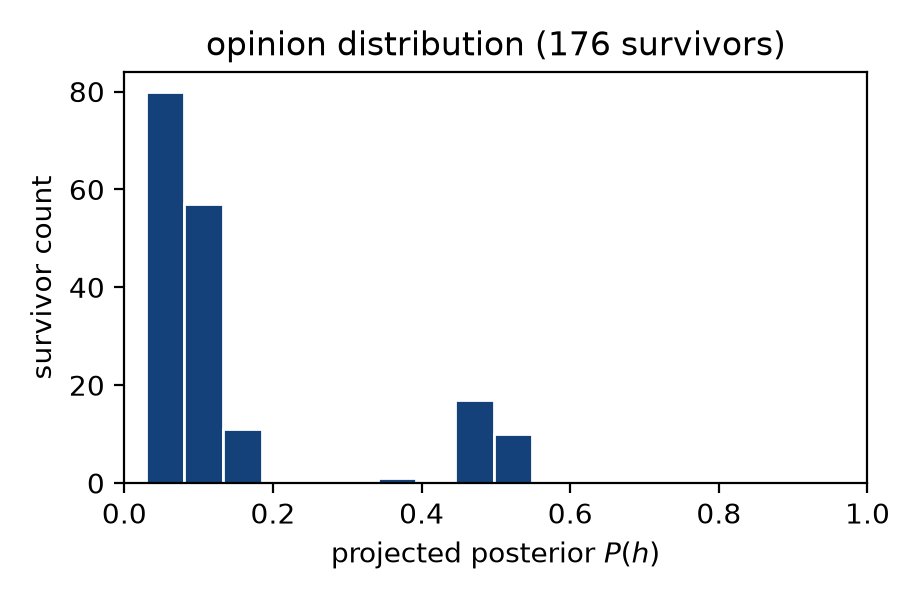
\includegraphics[width=0.62\linewidth]{figures/fig_opinion_histogram.png}
  \caption{Projected-posterior distribution across every distinct survivor named in \Cref{tab:bins}, generated by \texttt{figures/fig\_opinion\_histogram.py}.}
  \label{fig:opinion-hist}
\end{figure}

\begin{figure}[htbp]
  \centering
  
\includegraphics[width=0.92\linewidth]{figures/fig_bin_topk.png}
  \caption{Top-$k$ posterior ranking per time bin, generated by \texttt{figures/fig\_bin\_topk.py}.}
  \label{fig:bin-topk}
\end{figure}

\section{Calibration}
\label{sec:calibration}

This run held out evidence via 5-fold cross-validation (seed 0), scoring 105 held-out ground-truth events (17 covered by this run's own pre-holdout evidence) under belief constants $W=2.0$, $\lambda=0.50$. The resulting Brier score was 0.423. \Cref{tab:calibration} lists every non-empty reliability bin; \Cref{fig:calibration-curve} plots the same bins against the diagonal a perfectly calibrated run would sit on.

\begin{table}[htbp]
  \centering
  \caption{Discovery-date/k-fold holdout reliability bins.}
  \label{tab:calibration}
  \begin{tabular}{@{}lccc@{}}
    \toprule
    Predicted bin & Count & Mean predicted & Mean observed \\
    \midrule
    {[}0.0, 0.1{)} & 11 & 0.067 & 0.364 \\
    {[}0.1, 0.2{)} & 7 & 0.132 & 0.857 \\
    {[}0.2, 0.3{)} & 1 & 0.208 & 1.000 \\
    {[}0.3, 0.4{)} & 2 & 0.311 & 1.000 \\
    {[}0.4, 0.5{)} & 3 & 0.455 & 1.000 \\
    {[}0.5, 0.6{)} & 3 & 0.518 & 0.333 \\
    \bottomrule
  \end{tabular}
\end{table}

\begin{figure}[htbp]
  \centering
  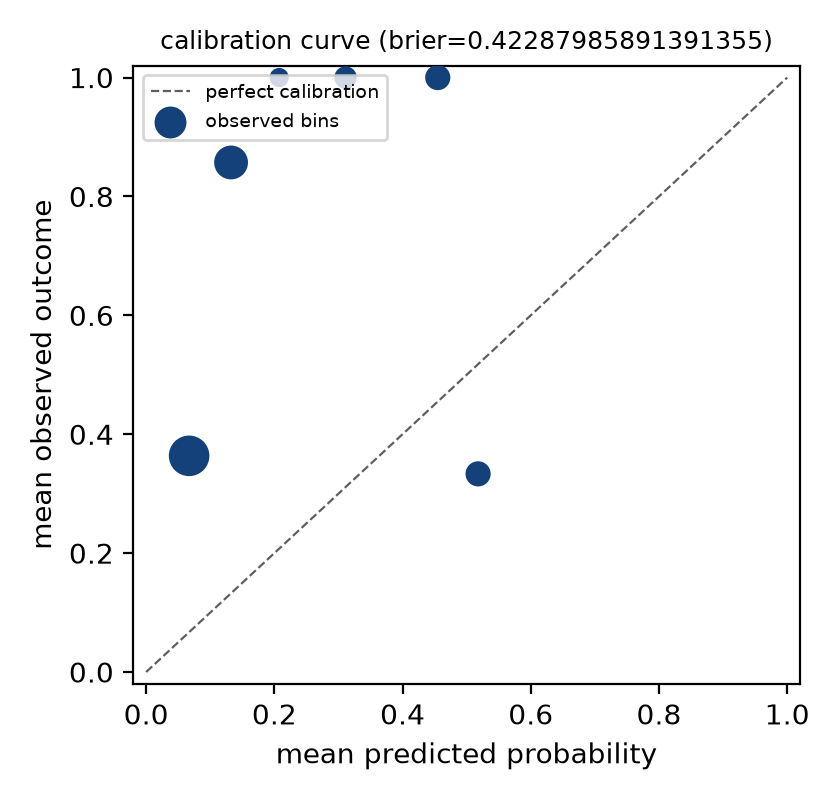
\includegraphics[width=0.55\linewidth]{figures/fig_calibration_curve.png}
  \caption{Discovery-date holdout reliability curve, generated by \texttt{figures/fig\_calibration\_curve.py}.}
  \label{fig:calibration-curve}
\end{figure}

\section{Limitations}
\label{sec:limitations}

Two of this run's own aggregates, robustness and surprise, are reported here only as the single scalar `MANIFEST.json` carries (\texttt{robustness\_stable\_fraction}, \texttt{surprise\_rate}); the per-hypothesis projections and the per-item surprise list that produced those scalars live only in the process's own memory during a run and are not written to any file this paper can read. A future run that persists them would let a later paper over this same campaign carry both as real tables instead.

The run's own self-report follows, quoted verbatim, exactly as the self-report role returned it: its assumptions, which slot vocabularies it judged incomplete, its missing-mass estimate, its calibration summary, and its target-blind check.
% voice-ignore-next 60
\begin{quote}\small
\begin{verbatim}
{
  "assumptions": [
    "Evidence volume (161 evidence items, 16 sources) is treated as 'stable' relative to the prior run since no prior-run source/evidence counts were supplied; the target_blind.steady=True flag is taken at face value as computed under that stability condition.",
    "The 11 vocab_added entries are treated as the full set of new terms introduced this run (no held-back or rejected proposals were reported), so vocabulary thinness is assessed purely from the rationale citations attached to each entry.",
    "coverage.missing_mass (0.03997) is treated as the primary point estimate; the reported coverage_low/coverage_high (0.023-0.031) is a narrower bootstrap band that does not bracket the point estimate, which is flagged as an internal inconsistency rather than silently reconciled.",
    "robustness_stable_fraction=1.0 is read as a survivor-level stability metric (176/176 hypotheses stable under perturbation), not as evidence that the vocabulary or opinion function itself is well-calibrated.",
    "The meta_review's 'lookup-table degeneracy' finding is treated as directly relevant to vocabulary-quality judgment: slots that don't move b/d/u when varied are functionally under-tested even if nominally populated."
  ],
  "incomplete_vocabularies": [
    "actor: all 4 new entries (Dowling and Milburn, Haroche and Wineland, Hanson group/TU Delft, EU Quantum Flagship) trace to just two narrative threads (T-2ndrev, T-belltests), each cited from a single claim/ms pointer - no independent corroborating source per actor, and meta_review confirms 'a' (authority) is actor-identity-locked rather than evidence-derived, so these actors enter the vocabulary without ever being evidentially stress-tested.",
    "mechanism: only 2 additions (single-system/single-quantum control; event-ready entanglement swapping), each from a single ms/claim pointer within the same two threads; meta_review shows uncertainty (u) is flat ~0.009-0.012 across the whole frontier regardless of mechanism, meaning these new mechanism labels have not yet produced any differentiated belief signal.",
    "action: 3 additions (crystallized, awarded a prize, closed a loophole) are the clearest case of cosmetic-only expansion - meta_review explicitly documents that dozens of hypotheses differing only in action/object share b/d/u to many decimal places, i.e. the action slot is populated but not discriminating in evaluation.",
    "object: 2 additions (second quantum revolution framing; loophole-free Bell test/NV-center swapping), same single-thread, single-citation sourcing as actor/mechanism above, and same non-discriminating-in-evaluation problem as action.",
    "place: only 1 addition (TU Delft) from a single ms pointer; meta_review separately flags that place exploration is heavily skewed (Planck/EPR clusters stuck on generic 'other-place'/'unknown-place', Solvay-Brussels over-generalized across an 82-year span), so the place vocabulary as a whole - not just this run's addition - is under-explored relative to its combinatorial importance (it appears to drive the one anomalous high-belief cluster)."
  ],
  "missing_mass_estimate": 0.04,
  "calibration_summary": "Calibration this run is weak: Brier score is 0.4229, well above the ~0.25 a trivial base-rate guesser would achieve on a binary-ish outcome space, and this sits alongside a modest surprise rate (0.130) and a meta-review that independently documents the mechanism behind the poor score - opinion outputs (b/d/u) are effectively keyed on (actor, place, mechanism, interval) rather than genuinely responsive to the action/object content that a third of this run's new vocabulary consists of, authority (a) tracks actor identity almost deterministically rather than evidence strength, and uncertainty (u) never leaves a narrow ~0.01 floor even for anachronistic or single-source claims. The one place the model deviates from its flat low-belief default (the solvay-brussels/[1927,2009] cluster) looks like an interval-width/place artifact rather than content-driven belief, per the meta-review's own flag. Net effect: robustness_stable_fraction=1.0 shows the survivor set is internally self-consistent under perturbation, but that stability is consistent with - and partly explained by - a collapsed, low-dimensional opinion function rather than genuine well-calibrated discrimination across the fuller hypothesis space implied by chao1_estimate (226,770 vs 5,990 observed).",
  "target_blind_steady": true,
  "target_blind_note": "The generator's non-consensus actor/mechanism proposal rate is reported at 0.95, identical to the prior run's 0.95 (steady=True, first_run=False), under what is assumed to be stable evidence volume. Read target-blind (i.e., without reference to whether those non-consensus proposals turned out surprising or high-belief), this is a healthy signal: the generator is not throttling back its willingness to propose actor/mechanism values outside the consensus set, mirroring how a stable surprise rate would indicate the evaluator isn't quietly drifting toward blandness. However, this steadiness should be read jointly with the vocabulary-thinness findings above: a steady 0.95 proposal rate for non-consensus values is reassuring about generator behavior, but it does not by itself certify that those non-consensus proposals are well-evidenced (most of this run's new actor/mechanism entries trace to single-citation pointers within only two of sixteen source threads) or that they are being evaluated with genuine content-sensitivity (per the meta-review's lookup-table-degeneracy and actor-locked-authority findings) - the health signal here is about generation, not about downstream evaluation quality."
}
\end{verbatim}
\end{quote}

\printbibliography

\appendix

\section{Glossary}
\label{app:glossary}

\printglossaryentry{opinion}
\printglossaryentry{posterior}
\printglossaryentry{missingmass}
\printglossaryentry{targetblind}
\printglossaryentry{coverageinterval}

\end{document}
